\subsubsection{Domain-klasse: Log}

Loggen har til formål at kunne lokalisere og identificere fejl i systemet. Loggen skal oprettes mere eller mindre globalt og der skal efterfølgende medgives en pointer til samtlige klasser på Pi. Alle disse klasser skal således anvende loggen som debugging redskab. Der skal som udgangspunkt kun skrives i loggen hvis en fejl opstår, da loggen ellers bliver uoverskuelig. Når der skrives til loggen, anvender den pågældende tråd cpu-tid, hvilket ligeledes er en grund til at være opmærksom på hvornår det er smart at skrive til loggen. \\
For at forhindre at log-entries fra forskellige tråde sammenflettes, skal der i implementeringen anvendes \texttt{std::mutex} som lås når der skrives i loggen.

\begin{figure}[h]
\centering
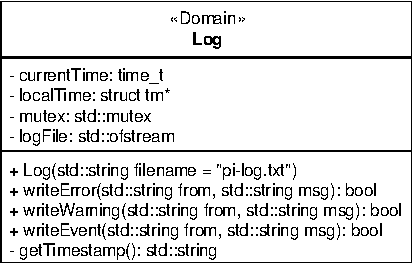
\includegraphics[]{../fig/diagrammer/bil/cd_log.pdf}
\caption{Klassebeskrivelse for domain-klassen Log}
\label{fig:cd_log}
\end{figure}

\textbf{Attributter}

\begin{table}[h]
\begin{tabularx}{\textwidth}{| Z | Z | L{10cm} |} \hline
Navn & Type & Beskrivelse \\\hline

\texttt{currentTime} & \texttt{time\_t} &Denne attribut bruges til at gemme det nuværende tidspunkt, når \texttt{getTimestamp} kaldes. \\\hline

\texttt{localTime} & \texttt{struct tm*} & Anvendes til at holde tiden i et læseligt format. \\\hline

\texttt{mutex} & \texttt{std::mutex} & Anvendes som lås i \texttt{std::lock\_guard} der forhindrer flere tråde i at skrive i loggen på samme tid. \\\hline

\texttt{logFile} & \texttt{std::ofstream} & File descriptor til logfilen. \\\hline

\end{tabularx}
\caption{Attributter for klassen Log}
\label{table:attr_log}
\end{table}


\textbf{Constructor}
%------------------------------------- Log -------------------------------------
\begin{table}[h]
\begin{tabularx}{\textwidth}{| L{2.5 cm} | Z |} \hline
Prototype & \texttt{Log(std::string filename = ''pi-log.txt'')} \\\hline
Parametre & \texttt{filename} \newline Det ønskede filnavn til logfilen der oprettes. Hvis denne parameter udelades ved initialiseringen bliver objektet oprettet med filnavnet ''pi-log.txt''.  \\\hline
Beskrivelse & Constructoren opretter et objekt af Log klassen med det angivne filnavn. \\\hline
\end{tabularx}
\caption{Beskrivelse af constructor for \texttt{Log}}
\label{table:con_log}
\end{table}

\clearpage

\textbf{Metoder}
%------------------------------------- writeError -------------------------------------
\begin{table}[h]
\begin{tabularx}{\textwidth}{| L{2.5 cm} | Z |} \hline
Prototype & \texttt{bool writeError(std::string from, std::string msg)} \\\hline
Parametre & \texttt{from} \newline Denne streng skal udfyldes med den indbyggede identifier ''\texttt{\_\_PRETTY\_FUNCTION\_\_}'' (GNU standard) der returnerer placeringen af det pågældende kald. Herved kan det i loggen ses præcis i hvilken klasse og metode log-beskeden kommer fra. \newline \newline \texttt{msg} \newline Den besked der skal stå i loggen. \\\hline
Returværdi &  \texttt{bool} \newline Returnerer \texttt{true} hvis skrivningen er gået godt og \texttt{false} hvis skrivningen gik galt. \\\hline
Beskrivelse & Metoden skriver en besked i loggen. Anvendes når der er sket en alvorlig fejl. \\\hline
\end{tabularx}
\caption{Metodebeskrivelse for \texttt{writeError}}
\label{table:met_writeError}
\end{table}

%------------------------------------- writeWarning -------------------------------------
\begin{table}[h]
\begin{tabularx}{\textwidth}{| L{2.5 cm} | Z |} \hline
Prototype & \texttt{bool writeWarning(std::string from, std::string msg)} \\\hline
Parametre & \texttt{from} \newline Denne streng skal udfyldes med den indbyggede identifier ''\texttt{\_\_PRETTY\_FUNCTION\_\_}'' (GNU standard) der returnerer placeringen af det pågældende kald. Herved kan det i loggen ses præcis i hvilken klasse og metode log-beskeden kommer fra. \newline \newline \texttt{msg} \newline Den besked der skal stå i loggen. \\\hline
Returværdi &  \texttt{bool} \newline Returnerer \texttt{true} hvis skrivningen er gået godt og \texttt{false} hvis skrivningen gik galt. \\\hline
Beskrivelse & Metoden skriver en besked i loggen. Anvendes når der er sket en mindre alvorlig fejl. \\\hline
\end{tabularx}
\caption{Metodebeskrivelse for \texttt{writeWarning}}
\label{table:met_writeWarning}
\end{table}

\clearpage

%------------------------------------- writeEvent -------------------------------------
\begin{table}[h]
\begin{tabularx}{\textwidth}{| L{2.5 cm} | Z |} \hline
Prototype & \texttt{bool writeEvent(std::string from, std::string msg)} \\\hline
Parametre & \texttt{from} \newline Denne streng skal udfyldes med den indbyggede identifier ''\texttt{\_\_PRETTY\_FUNCTION\_\_}'' (GNU standard) der returnerer placeringen af det pågældende kald. Herved kan det i loggen ses præcis i hvilken klasse og metode log-beskeden kommer fra. \newline \newline \texttt{msg} \newline Den besked der skal stå i loggen. \\\hline
Returværdi &  \texttt{bool} \newline Returnerer \texttt{true} hvis skrivningen er gået godt og \texttt{false} hvis skrivningen gik galt. \\\hline
Beskrivelse & Metoden skriver en besked i loggen. Anvendes når der er hændelse, der ikke er en fejl, som skal skrives i loggen. \\\hline
\end{tabularx}
\caption{Metodebeskrivelse for \texttt{writeEvent}}
\label{table:met_writeEvent}
\end{table}

%------------------------------------- getTimestamp -------------------------------------
\begin{table}[h]
\begin{tabularx}{\textwidth}{| L{2.5 cm} | Z |} \hline
Prototype & \texttt{std::string getTimestamp()} \\\hline
Parametre & ~ \newline \\\hline
Returværdi &  \texttt{std::string} \newline Returnerer en streng med systemets indstillede tid og dato. Formatet er \texttt{ÅÅÅÅ-MM-DD TT:MM:SS}.\\\hline
Beskrivelse & Metoden henter den nuværende tid i systemet og omdanner denne til en streng i en format der nemt kan anvendes i log-beskeder. \\\hline
\end{tabularx}
\caption{Metodebeskrivelse for \texttt{getTimestamp}}
\label{table:met_getTimestamp}
\end{table}